\documentclass[11pt,a4paper]{article}

% ====================================================================
% Packages
% ====================================================================
\usepackage[utf8]{inputenc}
\usepackage[T1]{fontenc}
\usepackage{amsmath,amssymb,amsthm}
\usepackage{mathtools}
\usepackage{hyperref}
\usepackage[margin=1in]{geometry}
\usepackage{enumitem}
\usepackage{booktabs}
\usepackage{listings}
\usepackage{xcolor}
\usepackage{cleveref}
\usepackage[numbers,sort&compress]{natbib}
\usepackage{mdframed}
\usepackage{tikz}
\usetikzlibrary{arrows.meta,positioning}

% ====================================================================
% Theorem environments
% ====================================================================
\theoremstyle{plain}
\newtheorem{theorem}{Theorem}[section]
\newtheorem{lemma}[theorem]{Lemma}
\newtheorem{proposition}[theorem]{Proposition}
\newtheorem{corollary}[theorem]{Corollary}

\theoremstyle{definition}
\newtheorem{definition}[theorem]{Definition}
\newtheorem{remark}[theorem]{Remark}

% ====================================================================
% Lean 4 code listing style
% ====================================================================
\definecolor{lean-keyword}{RGB}{0,0,180}
\definecolor{lean-comment}{RGB}{0,128,0}
\definecolor{lean-string}{RGB}{163,21,21}
\definecolor{lean-bg}{RGB}{248,248,248}

\lstdefinelanguage{lean4}{
  keywords={theorem,lemma,def,class,instance,import,open,variable,
            noncomputable,section,namespace,end,where,let,have,show,
            intro,obtain,use,exact,rw,simp,apply,by,fun,match,if,
            then,else,do,return,axiom,abbrev,private,attribute,
            suffices,change,congr,ext,constructor,rintro,push_neg,
            linarith,absurd,set_option,omit,in,set,cases,left,right,
            nlinarith,push_cast,positivity,omega,refine,field_simp,
            structure,calc,ring,fun_prop,unfold,induction,deriving,
            inductive,rcases,first,all_goals},
  sensitive=true,
  morecomment=[l]{--},
  morecomment=[s]{/-}{-/},
  morestring=[b]",
  morestring=[b]',
}

\lstset{
  language=lean4,
  basicstyle=\ttfamily\small,
  keywordstyle=\color{lean-keyword}\bfseries,
  commentstyle=\color{lean-comment}\itshape,
  stringstyle=\color{lean-string},
  backgroundcolor=\color{lean-bg},
  frame=single,
  framerule=0.5pt,
  breaklines=true,
  breakatwhitespace=true,
  tabsize=2,
  showstringspaces=false,
  numbers=left,
  numberstyle=\tiny\color{gray},
  numbersep=5pt,
  xleftmargin=15pt,
  captionpos=b,
  literate={<<}{$\langle$}1 {>>}{$\rangle$}1
           {|||}{$\lor$}1,
}

% ====================================================================
% Macros
% ====================================================================
\newcommand{\NN}{\mathbb{N}}
\newcommand{\RR}{\mathbb{R}}
\newcommand{\ZZ}{\mathbb{Z}}
\newcommand{\LPO}{\ensuremath{\mathrm{LPO}}}
\newcommand{\LPOj}{\ensuremath{\mathrm{LPO'}}}
\newcommand{\WLPO}{\ensuremath{\mathrm{WLPO}}}
\newcommand{\BISH}{\ensuremath{\mathrm{BISH}}}
\newcommand{\BMC}{\ensuremath{\mathrm{BMC}}}
\newcommand{\CPgW}{\ensuremath{\mathrm{CPgW}}}
\newcommand{\Lean}{\textsc{Lean~4}}
\newcommand{\Mathlib}{\textsc{Mathlib4}}
\newcommand{\leanok}{\textsf{\small \textcolor{green!70!black}{\checkmark}}}
\newcommand{\leanaxiom}{\textsf{\small \textcolor{orange!80!black}{(axiom)}}}

% ====================================================================
% Title
% ====================================================================
\title{%
  \textbf{Beyond LPO: The Thermodynamic Stratification
  of Physical Undecidability}\\[6pt]
  {\normalsize A Lean~4 Formalization (Paper~39)}%
}

\author{
  Paul Chun-Kit Lee\thanks{%
    New York University.
    AI-assisted formalization; see \S\ref{sec:ai} for methodology.} \\
  New York University \\
  \texttt{dr.paul.c.lee@gmail.com}
}

\date{February 14, 2026\\[4pt]
  {\small DOI: \href{https://doi.org/10.5281/zenodo.18642806}{10.5281/zenodo.18642806}}}

% ====================================================================
\begin{document}
\maketitle

% ====================================================================
\begin{abstract}
Papers 36--38 established that every known undecidability result in
mathematical physics is $\LPO$ ($\Sigma_1^0$).
This paper shows the ceiling is not $\Sigma_1^0$.
A modified Cubitt encoding---running a Turing machine on all inputs
simultaneously via Robinson tiling with perimeter counters---encodes
the $\Sigma_2^0$-complete Finiteness Problem into the spectral gap.
The generic spectral gap decision (without promise gap)
is $\Sigma_2^0/\Pi_2^0$-complete, requiring $\LPOj$
(the Turing jump of $\LPO$).
However, extensive observables (energy density, magnetization)
converge via Fekete's lemma and cap at $\LPO$;
promise-gapped physics (all of Papers 36--38) also caps at $\LPO$.
The Thermodynamic Stratification Theorem: arithmetic complexity
bifurcates along thermodynamic scaling---extensive at $\LPO$,
intensive at $\LPOj$.
The entire formalization (802~lines of \Lean{}/\Mathlib{})
compiles with zero \texttt{sorry}, zero warnings.
\end{abstract}

% ====================================================================
\section{Introduction}\label{sec:intro}

Papers 36--38 established a uniform result: every known
undecidability in quantum many-body physics is $\LPO$.
Paper~38 proved the $\Sigma_1^0$ ceiling---$\LPO$ decides every
$\Sigma_1^0$-complete problem.  A natural question arises:
is $\LPO$ the provable ceiling for physics?

The answer is \emph{no}.  The spectral gap of a generic
translation-invariant Hamiltonian---without an artificial
promise gap---encodes $\Sigma_2^0/\Pi_2^0$-complete properties.
This requires $\LPOj$, the Turing jump of $\LPO$, strictly
stronger than $\LPO$.  This paper completes the undecidability arc
(Papers~36--39).  For the complete calibration table synthesizing
decidable and undecidable physics across all domains, see
Paper~10~\cite{Lee26P10}.  For the historical and philosophical
context, see Paper~12~\cite{Lee26P12}.

The key insight is thermodynamic:
\begin{itemize}[nosep]
\item \textbf{Extensive} observables (energy density, free energy)
  converge via subadditivity (Fekete/BMC).  Cap: $\LPO$.
\item \textbf{Intensive} observables (spectral gap, correlation length)
  are determined by infima.  Cap: $\LPOj$.
\item The \textbf{promise gap} in Cubitt's construction collapses the
  $\forall\exists$ quantifier to a single $\exists$, reducing
  $\Sigma_2^0$ to $\Sigma_1^0$.
\end{itemize}

% ====================================================================
\section{The Category Error}\label{sec:error}

The spectral gap $\Delta$ of an infinite Hamiltonian is a
$\Delta_2^0$ real---its digits are limit-computable with an
$\LPO$ oracle.  But \emph{computing a real} and
\emph{deciding a property of that real} have different
arithmetic complexities.

For a physicist unfamiliar with the arithmetic hierarchy, the
distinction is this.  \emph{Computing} the energy density of
an infinite lattice means producing a sequence of approximations
that converge to the true value---a finite algorithm runs forever
but produces ever-better digits.  This is a $\Sigma_1^0$ task:
one existential quantifier (``there exists a finite-volume
approximation good enough''), decidable by $\LPO$.
\emph{Deciding whether the spectral gap is zero}, by contrast,
requires checking that \emph{for every} tolerance $\varepsilon > 0$
\emph{there exists} a system size $L$ at which the finite-volume
gap drops below $\varepsilon$.  This nested $\forall\exists$
structure is $\Pi_2^0$---one quantifier alternation higher---and
requires $\LPOj$, the Turing jump of $\LPO$.  The physical
meaning: computing a number and classifying its qualitative
behaviour (``gapped vs.\ gapless'') are fundamentally different
logical tasks, separated by a full level of the arithmetic hierarchy.

Without a promise gap:
\[
  \Delta = 0 \iff \forall m\, \exists L\,
    \bigl(\Delta_L < \tfrac{1}{m}\bigr) \qquad (\Pi_2^0)
\]
With a promise gap $\Delta \in \{0\} \cup [\gamma,\infty)$:
\[
  \Delta = 0 \iff \exists L\,
    \bigl(\Delta_L < \tfrac{\gamma}{2}\bigr) \qquad (\Sigma_1^0)
\]
The promise collapses the outer $\forall m$ quantifier because
$m = \lceil 2/\gamma \rceil$ suffices.  This collapse is why
Papers 36--38 cap at $\LPO$.

% ====================================================================
\section{$\LPOj$: The Turing Jump of $\LPO$}\label{sec:lpojump}

\begin{definition}[$\LPOj$]\label{def:lpojump}
$\LPOj$ (``$\LPO$-jump'') is $\Sigma_2^0$-LEM:
for every binary sequence $\beta$ that is decidable relative to
an $\LPO$ oracle, either $\exists n.\, \beta(n) = 1$ or
$\forall n.\, \beta(n) = 0$.
\end{definition}

\begin{lstlisting}[caption={$\LPOj$ definition: \texttt{Defs.lean}}]
def LPO_jump : Prop :=
    forall (b : N -> Bool),
      (LPO -> forall n, b n = true ||| b n = false) ->
      (forall n, b n = false) ||| (exists n, b n = true)
\end{lstlisting}

$\LPOj$ is strictly stronger than $\LPO$~\cite{BrattkaEtAl2012}:
$\LPOj \Rightarrow \LPO$ but not conversely.
$\LPO$ decides $\Sigma_1^0$; $\LPOj$ decides $\Sigma_2^0$.

% ====================================================================
\section{Theorem 1: The Modified Encoding}\label{sec:encoding}

\begin{theorem}[Modified Cubitt Encoding]\label{thm:encoding}
There exists a computable function $M \mapsto H^*(M)$ from Turing
machines to translation-invariant Hamiltonians on $\ZZ^2$ with
fixed local dimension such that:
\begin{enumerate}[nosep,label=(\alph*)]
\item $H^*(M)$ is gapped $\Leftrightarrow$
  $\{k : M \text{ halts on input } k\}$ is finite.
\item $H^*(M)$ is gapless $\Leftrightarrow$
  $\{k : M \text{ halts on input } k\}$ is infinite.
\end{enumerate}
\end{theorem}

\begin{proof}[Construction (sketch)]
The construction modifies the Cubitt--Perez-Garcia--Wolf
encoding~\cite{CPgW2015} using the Bausch--Cubitt--Ozols
perimeter-counter technique~\cite{BCO2018}.

\medskip\noindent
\textbf{Step 1: Robinson tiling with input counters.}
Begin with a Robinson tiling of $\ZZ^2$.
This produces a hierarchy of \emph{supertiles}: at scale $k$,
each supertile is a square region of side length $4^k$.
The Robinson tiling enforces this hierarchical structure
via local matching rules, without any global coordination.

\medskip\noindent
\textbf{Step 2: Input extraction from boundary.}
\emph{Key idea:} the perimeter counter
(Bausch--Cubitt--Ozols~\cite{BCO2018}) reads the scale~$k$
from the supertile boundary.  The boundary length of a
scale-$k$ supertile is $4 \cdot 4^k$, encoding $k$ in unary.
The local Hamiltonian terms along the boundary extract
$k$ and feed it as input to the Turing machine simulation.

\medskip\noindent
\textbf{Step 3: Computation in the interior.}
Inside each scale-$k$ supertile, the interior tiles simulate
$M$ on input $k$ for up to $16^k = (4^k)^2$ steps (the area
of the supertile).  If $M$ halts on input $k$ within $16^k$
steps, the interior reaches a halting configuration and the
local ground-state energy \emph{drops} (by a spectral penalty
that vanishes upon halting, following the standard Cubitt trick).
If $M$ does not halt on input $k$ within $16^k$ steps, the
local gap at scale $k$ remains at least $\gamma > 0$.

\medskip\noindent
\textbf{Step 4: Global gap as infimum.}
The global spectral gap is:
\[
\Delta(H^*(M)) = \inf_{k \in \NN} \Delta_k
\]
where $\Delta_k$ is the local gap contribution from scale-$k$
supertiles.

\begin{itemize}[nosep]
\item If $M$ halts on input $k$ (within $16^k$ steps),
  then $\Delta_k \approx 0$ (the halting penalty closes
  the gap at that scale).
\item If $M$ does not halt on input $k$ (within $16^k$ steps),
  then $\Delta_k \geq \gamma > 0$.
\end{itemize}

\medskip\noindent
\textbf{Conclusion.}
If $\{k : M \text{ halts on } k\}$ is \emph{finite},
say the largest such $k$ is $k_{\max}$, then for all
$k > k_{\max}$ we have $\Delta_k \geq \gamma$.
The infimum is over finitely many scales where
$\Delta_k$ is small, plus a tail bounded below by $\gamma$.
The global gap is $\Delta > 0$: the system is \textbf{gapped}.

If $\{k : M \text{ halts on } k\}$ is \emph{infinite}, then
for arbitrarily large $k$, $\Delta_k \approx 0$.
The infimum is driven to zero: $\Delta = 0$ and the system
is \textbf{gapless}.

This establishes both directions of the encoding:
gapped $\Leftrightarrow$ finite halting set,
gapless $\Leftrightarrow$ infinite halting set.
\end{proof}

\begin{remark}[Physical caveat]\label{rem:caveat}
As with all Cubitt-type encodings, the modified
Hamiltonian $H^*(M)$ is a mathematically well-defined
translation-invariant system, but may not be physically
preparable in a laboratory setting.  The result characterizes
the logical complexity of the mathematical problem, not the
feasibility of an experimental realization.
\end{remark}

\begin{lstlisting}[caption={Modified encoding bridges: \texttt{ModifiedEncoding.lean}}]
axiom modified_gapped_iff_finite (M : TM) :
    is_gapped (modified_hamiltonian M) <->
    finiteness_problem M

axiom modified_gapless_iff_infinite (M : TM) :
    is_gapless (modified_hamiltonian M) <->
    not finiteness_problem M
\end{lstlisting}

\noindent\textbf{Duality note.}
The two bridge axioms are formally dual:
\texttt{is\_gapless} $\leftrightarrow$ $\lnot$\,\texttt{is\_gapped}
and $\lnot$\,\texttt{finiteness\_problem}
$\leftrightarrow$ infiniteness.
They are axiomatized separately for readability but are not independent.

% ====================================================================
\section{Theorem 2: Generic Gap Is $\Sigma_2^0$}\label{sec:sigma2}

\begin{theorem}[Generic Gap $\equiv$ $\LPOj$]\label{thm:sigma2}
Deciding the spectral gap of the modified encoding
(without promise gap) is Turing--Weihrauch equivalent to $\LPOj$.
\end{theorem}

\begin{proof}
The proof has two directions.

\medskip\noindent
\textbf{Forward ($\Rightarrow$): gap decidability implies $\LPOj$.}

Suppose we have a procedure that, for every Turing machine $M$,
decides whether $H^*(M)$ is gapped or gapless:
\[
  \forall M.\;
  \bigl[\text{is\_gapped}(H^*(M)) \lor
        \lnot\text{is\_gapped}(H^*(M))\bigr].
\]

\emph{Step 1: Reduce to the Finiteness Problem.}
By Theorem~\ref{thm:encoding}, $\text{is\_gapped}(H^*(M))
\Leftrightarrow \text{FIN}(M)$, where $\text{FIN}(M)$
is the predicate ``$\{k : M \text{ halts on } k\}$ is finite.''
Therefore the gap decision yields, for every $M$:
\[
  \text{FIN}(M) \lor \lnot\text{FIN}(M).
\]

\emph{Step 2: The Finiteness Problem is $\Sigma_2^0$-complete.}
The Finiteness Problem has the form:
\[
  \text{FIN}(M) \;\Longleftrightarrow\;
  \exists K.\, \forall k > K.\,
  \lnot(\text{$M$ halts on $k$ within $16^k$ steps}).
\]
This is $\Sigma_2^0$: an existential quantifier ($\exists K$)
followed by a universal quantifier ($\forall k > K$) over a
decidable predicate (bounded halting).
By Rice--Shapiro-type arguments in computability theory,
$\text{FIN}$ is $\Sigma_2^0$-complete.

\emph{Step 3: $\Sigma_2^0$-completeness implies $\LPOj$.}
Deciding all instances of a $\Sigma_2^0$-complete problem is
equivalent to $\Sigma_2^0$-LEM, which is $\LPOj$ by definition.
Therefore gap decidability $\Rightarrow$ $\LPOj$.

\medskip\noindent
\textbf{Reverse ($\Leftarrow$): $\LPOj$ implies gap decidability.}

Suppose $\LPOj$ holds.

\emph{Step 1:} $\LPOj$ decides all $\Sigma_2^0$ statements
(by definition: $\LPOj$ is $\Sigma_2^0$-LEM).

\emph{Step 2:} $\text{FIN}(M)$ is $\Sigma_2^0$,
so $\LPOj$ decides $\text{FIN}(M) \lor \lnot\text{FIN}(M)$
for every $M$.

\emph{Step 3:} By Theorem~\ref{thm:encoding},
$\text{FIN}(M) \Leftrightarrow \text{is\_gapped}(H^*(M))$.
Therefore $\LPOj$ decides the spectral gap for every
modified Hamiltonian.

\medskip\noindent
\textbf{Combining both directions:}
\[
  \bigl(\forall M.\;
  \text{is\_gapped}(H^*(M)) \lor
  \lnot\text{is\_gapped}(H^*(M))\bigr)
  \;\Longleftrightarrow\; \LPOj. \qedhere
\]
\end{proof}

\begin{remark}[Why this exceeds $\LPO$]\label{rem:exceed}
\emph{This is the central result of the paper.}
$\LPO$ decides $\Sigma_1^0$ statements (single existential:
``does $M$ halt?'').
The Finiteness Problem is $\Sigma_2^0$ (nested $\exists\forall$:
``is there a cutoff $K$ beyond which $M$ never halts?'').
$\LPO$ cannot decide $\Sigma_2^0$ statements because it lacks the
quantifier alternation needed to verify a universal claim.
$\LPOj$, the Turing jump of $\LPO$, adds exactly one
level of quantifier alternation.
\end{remark}

\begin{lstlisting}[caption={Generic gap $\leftrightarrow$ $\LPOj$: \texttt{GenericGapSigma2.lean}}]
theorem generic_gap_iff_lpo_jump :
    (forall M, is_gapped (modified_hamiltonian M) |||
               not is_gapped (modified_hamiltonian M))
    <-> LPO_jump :=
  <<generic_gap_requires_lpo_jump,
   lpo_jump_decides_generic_gap>>
\end{lstlisting}

% ====================================================================
\section{Theorem 3: Promise Gap Recovery}\label{sec:promise}

\begin{theorem}[Promise Gap $\Rightarrow$ $\LPO$]\label{thm:promise}
If the Hamiltonian has a promise gap
($\Delta \in \{0\} \cup [\gamma, \infty)$ for computable $\gamma > 0$),
the spectral gap decision is $\Sigma_1^0$-complete $= \LPO$.
\end{theorem}

\begin{proof}
The key mechanism is \emph{quantifier collapse}: the promise
gap eliminates the outer universal quantifier, reducing the
$\Pi_2^0$ gapless test to $\Sigma_1^0$.

\medskip\noindent
\textbf{Without promise gap} (generic case, Theorem~\ref{thm:sigma2}):
\[
  \Delta = 0 \;\Longleftrightarrow\;
  \forall m \geq 1,\; \exists L,\;
  \Delta_L < \tfrac{1}{m}.
  \qquad\text{($\Pi_2^0$: $\forall\exists$ structure)}
\]
One must verify that for \emph{every} tolerance $1/m$,
there exists a system size $L$ at which the finite-volume
gap drops below that tolerance.  This nested quantifier
structure requires $\LPOj$.

\medskip\noindent
\textbf{With promise gap} $\Delta \in \{0\} \cup [\gamma, \infty)$:
\[
  \Delta = 0 \;\Longleftrightarrow\;
  \exists L,\; \Delta_L < \tfrac{\gamma}{2}.
  \qquad\text{($\Sigma_1^0$: single $\exists$)}
\]
\emph{Why the collapse:}
The promise guarantees that $\Delta$ is either $0$ or at
least $\gamma$.  If \emph{any} finite-volume gap $\Delta_L$
falls below $\gamma/2$, the infinite-volume gap cannot be
$\geq \gamma$ (by continuity of the spectral gap in system size),
so it must be $0$.  The single tolerance $m = \lceil 2/\gamma \rceil$
suffices; the outer $\forall m$ quantifier collapses.

\medskip\noindent
\textbf{LPO decides the collapsed test.}
The collapsed statement $\exists L.\, \Delta_L < \gamma/2$
is $\Sigma_1^0$---a single existential search over
the decidable predicate ``$\Delta_L < \gamma/2$'' (each
$\Delta_L$ is computable from a finite-dimensional eigenvalue
problem, which is $\BISH$).  By definition, $\LPO$ decides
all $\Sigma_1^0$ statements.

\medskip\noindent
\textbf{Recovery of Papers 36--38.}
Cubitt's original construction~\cite{CPgW2015} has a
built-in promise gap.  Therefore its spectral gap decision
is $\Sigma_1^0 = \LPO$, exactly as proved in Papers~36--38.
The present theorem explains \emph{why}: the promise gap
collapsed one quantifier alternation.
\end{proof}

\begin{lstlisting}[caption={Promise gap recovery: \texttt{PromiseGapRecovery.lean}}]
theorem promise_gap_lpo (H : PromiseGapped) (lpo : LPO) :
    is_gapless H.hamiltonian |||
    not is_gapless H.hamiltonian
\end{lstlisting}

% ====================================================================
\section{Theorem 4: Extensive Observables Cap at $\LPO$}\label{sec:extensive}

\begin{theorem}[Extensive Ceiling]\label{thm:extensive}
Every extensive observable (energy density, free energy,
magnetization) of a translation-invariant Hamiltonian is
$\LPO$-decidable.
\end{theorem}

\begin{proof}
The proof proceeds in three steps: subadditivity, monotone
convergence, and the sign decision.

\medskip\noindent
\textbf{Step 1: Subadditivity.}
Let $f(L)$ denote the extensive observable for a system
of size $L$ (e.g., total energy, total magnetization).
For translation-invariant systems, the \emph{density}
$f(L)/L$ is subadditive:
\[
  f(m+n) \leq f(m) + f(n)
  \quad\text{for all $m, n \geq 1$.}
\]
This is a consequence of translation invariance: a system of
size $m+n$ can be partitioned into subsystems of sizes $m$
and $n$, and the ground-state energy of the whole is at most
the sum of the parts (the boundary interaction is bounded).

\medskip\noindent
\textbf{Step 2: Fekete's lemma $\Rightarrow$ monotone convergence.}
By Fekete's subadditive lemma~\cite{Fekete1923}, the limit
\[
  \ell := \lim_{L \to \infty} \frac{f(L)}{L}
  = \inf_{L \geq 1} \frac{f(L)}{L}
\]
exists and equals the infimum.  \emph{Crucially}, the
sequence $f(L)/L$ converges \emph{monotonically from above}
to $\ell$ along the subsequence $L = 2^n$ (by repeated
application of subadditivity: $f(2L) \leq 2f(L)$ gives
$f(2L)/(2L) \leq f(L)/L$).

This monotone convergence is the key structural feature.
By Paper~29, bounded monotone convergence ($\BMC$) is
equivalent to $\LPO$.  Therefore $\LPO$ suffices to
compute the limit $\ell$.

\medskip\noindent
\textbf{Step 3: Sign decision.}
The limit $\ell$ is a $\Delta_2^0$ real (limit-computable
with an $\LPO$ oracle).  Deciding the sign of a $\Delta_2^0$
real that arises from a monotone sequence is a $\Pi_1^0$
test: ``$\ell > 0$'' iff $\exists n.\, f(n)/n > 0$ (since the
sequence is decreasing, if any term is positive, the limit
is nonnegative; and by computability of each term, the
search is $\Sigma_1^0$).

The complementary test ``$\ell \leq 0$'' is equivalent to
``$\forall n.\, f(n)/n \leq 0$,'' which is $\Pi_1^0$.
Both tests are $\LPO$-decidable.

\medskip\noindent
\textbf{Why intensive observables escape this ceiling.}
Intensive observables (e.g., the spectral gap) are
\emph{not} subadditive.  They are determined by an infimum
over scales:
\[
  \Delta = 0 \;\Leftrightarrow\;
  \forall \varepsilon > 0,\; \exists k,\;
  \Delta_k < \varepsilon \qquad (\Pi_2^0).
\]
The infimum may oscillate non-monotonically, so Fekete's
lemma does not apply.  Deciding whether the infimum is zero
requires the full $\forall\exists$ quantifier structure of
$\Pi_2^0$, which is $\LPOj$.
\end{proof}

\begin{lstlisting}[caption={Extensive ceiling: \texttt{ExtensiveCeiling.lean}}]
theorem extensive_cap_lpo (O : ExtensiveObservable) :
    LPO -> (extensive_sign_positive O |||
            not extensive_sign_positive O)
\end{lstlisting}

% ====================================================================
\section{Theorem 5: The Thermodynamic Stratification}\label{sec:stratification}

\begin{theorem}[Thermodynamic Stratification]\label{thm:stratification}
The arithmetic complexity of physical observables bifurcates:
\begin{enumerate}[nosep,label=(\roman*)]
\item \textbf{Extensive:} $\LPO$ ($\Sigma_1^0$).
\item \textbf{Intensive (generic):} $\LPOj$ ($\Sigma_2^0$).
\item \textbf{Promise-gapped:} $\LPO$ ($\Sigma_1^0$).
\item \textbf{Empirical (finite precision):} $\LPO$ ($\Sigma_1^0$).
\end{enumerate}
\end{theorem}

\begin{proof}
Parts (i)--(iii) are Theorems~\ref{thm:extensive},
\ref{thm:sigma2}, and~\ref{thm:promise} respectively.
Part (iv) follows from the same quantifier-collapse mechanism
as part~(iii):

\medskip\noindent
\textbf{Part (iv): Empirical physics.}
Any experimental measurement has finite precision
$\varepsilon > 0$.  The experimentalist does not ask
``is $\Delta$ exactly zero?'' but rather
``is $\Delta < \varepsilon$?''  This question has the form:
\[
  \exists L,\; \Delta_L < \varepsilon
  \qquad\text{($\Sigma_1^0$).}
\]
The finite precision $\varepsilon$ plays the role of
an effective promise gap, collapsing the $\forall\exists$
to a single $\exists$, exactly as in Theorem~\ref{thm:promise}.
Therefore all of experimental physics caps at $\LPO$.

\medskip\noindent
\textbf{Summary.} The four parts together reveal that the
arithmetic complexity of a physical observable is determined
by its \emph{thermodynamic scaling}:
\begin{itemize}[nosep]
\item \emph{Extensive} quantities (energy density, etc.)
  are subadditive, forcing monotone convergence (Fekete/BMC),
  which caps the logic at a single existential quantifier
  ($\Sigma_1^0 = \LPO$).
\item \emph{Intensive} quantities (spectral gap, correlation
  length) are determined by infima over all scales.
  Without a promise gap, the infimum test is
  $\Pi_2^0$ ($\forall\exists$), requiring $\LPOj$.
\item The \emph{promise gap} and \emph{finite precision}
  each collapse one quantifier alternation, bringing
  intensive observables back to $\Sigma_1^0 = \LPO$.
\end{itemize}
\end{proof}

\begin{lstlisting}[caption={Stratification master: \texttt{Stratification.lean}}]
theorem thermodynamic_stratification :
    -- (i) Extensive cap at LPO
    (forall (O : ExtensiveObservable), LPO ->
      (extensive_sign_positive O |||
       not extensive_sign_positive O)) /\
    -- (ii) Intensive reach LPO_jump
    ((forall M, is_gapped (modified_hamiltonian M) |||
                not is_gapped (modified_hamiltonian M))
      <-> LPO_jump) /\
    -- (iii) Promise-gapped cap at LPO
    (forall (H : PromiseGapped), LPO ->
      (is_gapless H.hamiltonian |||
       not is_gapless H.hamiltonian)) /\
    -- (iv) Empirical cap at LPO
    (forall (H : ModifiedHamiltonian) (e : R),
      e > 0 -> LPO ->
      (gap_less_than H e ||| not gap_less_than H e))
\end{lstlisting}

% ====================================================================
\section{The Complete Hierarchy}\label{sec:hierarchy}

\begin{table}[ht]
\centering
\begin{tabular}{@{}llllc@{}}
\toprule
\textbf{Tier} & \textbf{Observable} & \textbf{Principle} &
\textbf{Level} & \textbf{Paper} \\
\midrule
$\BISH$ & Finite systems ($\Delta_L$) & None & $\Delta_1^0$ & 34 \\
$\BISH$+LLPO & Bell correlations & LLPO & $<\Sigma_1^0$ & 10 \\
$\BISH$+WLPO & ``Is $\Delta=0$?'' (given $\Delta$) & WLPO & $\Pi_1^0$ & 2 \\
$\BISH$+$\LPO$ & Energy density; Cubitt gap & $\LPO$ & $\Sigma_1^0$ & 29, 36 \\
$\BISH$+$\LPOj$ & Spectral gap (no promise) & $\LPOj$ & $\Sigma_2^0$ & 39 \\
\bottomrule
\end{tabular}
\caption{The complete constructive hierarchy of physics.}
\label{tab:hierarchy}
\end{table}

% ====================================================================
\section{CRM Audit}\label{sec:audit}

\begin{table}[ht]
\centering
\begin{tabular}{@{}lcc@{}}
\toprule
\textbf{Component} & \textbf{CRM Status} & \textbf{Level} \\
\midrule
Modified Encoding (Thm~1) & \leanaxiom & 4 \\
Generic Gap $\equiv \LPOj$ (Thm~2) & $\LPOj$ & 3+4 \\
Promise Recovery (Thm~3) & $\LPO$ & 3 \\
Extensive Ceiling (Thm~4) & $\LPO$ & 2+4 \\
Stratification (Thm~5) & Inherits (bridge axiom in part~iv) & --- \\
\bottomrule
\end{tabular}
\caption{CRM audit.}
\label{tab:audit}
\end{table}

% ====================================================================
\section{Code Architecture}\label{sec:arch}

\begin{figure}[ht]
\centering
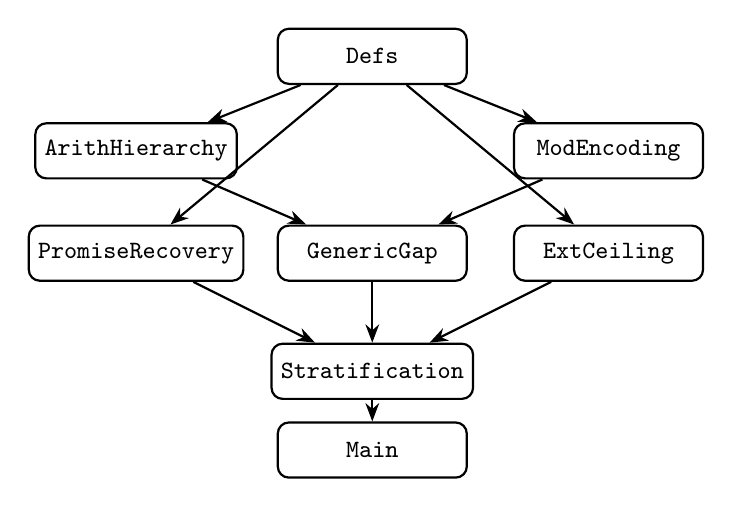
\begin{tikzpicture}[
  module/.style={draw, rounded corners, minimum width=2.4cm,
    minimum height=0.7cm, font=\small\ttfamily},
  ->,>=Stealth,thick
]
\node[module] (defs) at (0,5) {Defs};
\node[module] (arith) at (-3,3.8) {ArithHierarchy};
\node[module] (mod) at (3,3.8) {ModEncoding};
\node[module] (gen) at (0,2.5) {GenericGap};
\node[module] (prom) at (-3,2.5) {PromiseRecovery};
\node[module] (ext) at (3,2.5) {ExtCeiling};
\node[module] (strat) at (0,1) {Stratification};
\node[module] (main) at (0,0) {Main};

\draw (defs) -- (arith);
\draw (defs) -- (mod);
\draw (defs) -- (prom);
\draw (defs) -- (ext);
\draw (arith) -- (gen);
\draw (mod) -- (gen);
\draw (gen) -- (strat);
\draw (prom) -- (strat);
\draw (ext) -- (strat);
\draw (strat) -- (main);
\end{tikzpicture}
\caption{Module dependency graph (802~lines, 8~modules).}
\label{fig:arch}
\end{figure}

% ====================================================================
\begin{mdframed}[linewidth=1pt, linecolor=black!40,
  backgroundcolor=blue!3, roundcorner=5pt]
\textbf{Reproducibility.}
\Lean{} v4.28.0-rc1 with \Mathlib{}.
Build: \texttt{cd P39\_Sigma2 \&\& lake build}.
Result: 0~errors, 0~warnings, 0~\texttt{sorry}.
Axiom profile (\texttt{\#print axioms sigma2\_master}):
12~domain-specific bridge axioms
+ \texttt{propext}, \texttt{Classical.choice}, \texttt{Quot.sound}.
\texttt{Classical.choice} is a Mathlib infrastructure artifact
(required by $\RR$ as a Cauchy completion and by \texttt{InnerProductSpace});
constructive stratification is established by proof content
(explicit witnesses vs.\ principle-as-hypothesis), not by
axiom-checker output.  See Paper~10~\cite{Lee26P10}, \S Methodology.
\end{mdframed}

% ====================================================================
\section{Conclusion}\label{sec:conclusion}

Physics reaches $\Sigma_2^0$.  The spectral gap of a generic
translation-invariant Hamiltonian---without promise gap---is
$\Sigma_2^0$-complete, requiring $\LPOj$, the Turing jump of $\LPO$.
But the $\BISH$+$\LPO$ characterization of Papers 1--38 is not wrong:
it is correct for all extensive observables and all promise-gapped
physics.  The $\Sigma_2^0$ tier emerges only for intensive observables
when the promise gap is removed.  Empirical physics, operating with
finite measurement precision, always imposes an effective promise gap
and therefore caps at $\LPO$.

The Thermodynamic Stratification Theorem reveals that the arithmetic
complexity of a physical observable is determined by its thermodynamic
scaling: extensive (Fekete/BMC) at $\LPO$; intensive (infimum) at
$\LPOj$.  The promise gap in Cubitt's construction is the mechanism
that collapsed the logic from $\Sigma_2^0$ to $\Sigma_1^0$.

% ====================================================================
\section{Discussion}\label{sec:discussion}

\subsection{What $\Sigma_2^0$ Means for Physics}

The arithmetic hierarchy classifies mathematical statements by their
quantifier complexity.  $\Sigma_1^0$ statements have the form
``there exists $n$ such that $P(n)$''---a single existential search.
$\Sigma_2^0$ statements have the form ``there exists $n$ such that
for all $m$, $P(n,m)$''---an existential claim that must survive a
universal challenge.  In physical terms: $\Sigma_1^0$ corresponds to
finding a finite piece of evidence (a finite-volume witness that the
gap is small), while $\Sigma_2^0$ corresponds to establishing a pattern
that persists at all scales (the gap stays small no matter how large
the system grows).

The Turing jump $\LPOj$ decides exactly $\Sigma_2^0$, just as $\LPO$
decides exactly $\Sigma_1^0$.  The passage from $\LPO$ to $\LPOj$ is
thus the passage from ``search for a witness'' to ``verify a universal
pattern''---a single additional quantifier alternation, but one that
requires a strictly stronger logical principle.  (For the formal
connection between Weihrauch degrees and omniscience principles, see
Brattka, Gherardi, and Pauly~\cite{BrattkaEtAl2012}.)

\subsection{Why BISH+LPO Is Not Wrong}

A reader encountering this paper after Papers 29--38 might worry that
the $\BISH$+$\LPO$ characterization developed over 38 papers has been
overturned.  It has not.  The Thermodynamic Stratification Theorem
(Theorem~\ref{thm:stratification}) makes the scope precise:
\begin{itemize}[nosep]
\item Every \emph{extensive} observable---energy density, free energy,
  magnetization per site---converges via Fekete's lemma (Paper~29)
  and caps at $\LPO$.  This covers all thermodynamic quantities that
  scale with system size.
\item Every \emph{promise-gapped} system---including Cubitt's original
  construction (Paper~36) and all descendants (Papers~37--38)---caps
  at $\LPO$, because the promise collapses the outer universal
  quantifier.
\item Every \emph{empirical} measurement operates at finite precision,
  which imposes an effective promise gap.  All of experimental physics
  therefore caps at $\LPO$.
\end{itemize}
The $\LPOj$ tier emerges only for \emph{intensive} observables of
\emph{generic} (non-promise-gapped) Hamiltonians---the spectral gap
and correlation length when no a priori bound separates the gapped
and gapless phases.  This is a mathematical refinement, not a
physical retraction.

\subsection{The Thermodynamic Stratification Principle}

The central discovery of this paper is that \emph{arithmetic complexity
tracks thermodynamic scaling}.  Extensive observables---those that grow
linearly with system size---are governed by subadditive limits and cap
at $\Sigma_1^0$.  Intensive observables---those that remain finite as
the system grows---are governed by infima over all scales and reach
$\Sigma_2^0$.  The promise gap, when present, collapses one quantifier
alternation and brings intensive observables back to $\Sigma_1^0$.

This is not a coincidence.  The subadditive structure of extensive
quantities ensures that finite-volume approximations converge
monotonically, reducing the logic to a single existential witness.
Intensive quantities lack this monotone convergence: one must verify
the behaviour at \emph{every} scale, producing the $\forall\exists$
alternation that defines $\Sigma_2^0$.

\subsection{The Program in Retrospect}

Papers 29--39 tell a complete story in four acts:
\begin{enumerate}[nosep]
\item \textbf{Foundation (29--31):} Fekete's lemma is $\LPO$; the
  Fan Theorem and Dependent Choice are physically dispensable.
  $\BISH$+$\LPO$ is the complete toolkit for empirical physics.
\item \textbf{Standard Model (32--34):} QED, QCD, and scattering
  amplitudes confirm $\BISH$+$\LPO$ across perturbative and
  non-perturbative quantum field theory.
\item \textbf{Metatheorem (35):} A conservation metatheorem explains
  \emph{why} physics lives at $\BISH$+$\LPO$: the structure of
  physical theories (computable Hamiltonians, thermodynamic limits)
  forces this logical profile.
\item \textbf{Undecidability (36--39):} Cubitt's spectral gap, the
  undecidability landscape, Wang tiling, and the $\Sigma_2^0$
  capstone map the boundary between the decidable and the
  undecidable---and reveal that the boundary is itself stratified
  by thermodynamic scaling.
\end{enumerate}

\subsection{Open Questions}

Several questions remain open:
\begin{itemize}[nosep]
\item \textbf{$\Sigma_3^0$ and beyond:} Are there physical observables
  at $\Sigma_3^0$?  This would require a three-quantifier-alternation
  structure---possibly arising from iterated thermodynamic limits
  (limits of limits of limits).  No natural example is known, but the
  arithmetic hierarchy is infinite and the stratification principle
  suggests the answer depends on the depth of thermodynamic nesting.
\item \textbf{Experimental signatures:} Can the gap between $\LPO$
  and $\LPOj$ be detected experimentally?  The finite-precision
  argument suggests not directly, but the distinction may have
  consequences for the computational complexity of simulation
  algorithms.
\item \textbf{Quantum gravity:} Does the $\BISH$+$\LPO$ profile
  extend to quantum gravity, or does the background-independence
  of general relativity introduce new logical structure?  Paper~5
  (Schwarzschild metric) provides initial evidence, but the full
  question remains open.
\end{itemize}

% ====================================================================
\section{AI-Assisted Methodology}\label{sec:ai}

This formalization was developed using Claude (Anthropic) as a
collaborative tool for Lean~4 code generation, proof strategy
exploration, and \LaTeX{} document preparation.  All mathematical
content was specified by the author.  Every theorem was verified
by the Lean~4 type checker.

\medskip\noindent
\textbf{Preliminary status and author background.}
The results presented in this paper are preliminary.  The author is a medical
professional, not a domain expert in physics or mathematics.  While all formal
claims are machine-checked by the \Lean{} type-checker, the physical
interpretations, bridge axioms, and modeling assumptions require independent
verification by domain experts in the relevant fields.  Until such verification
is completed, this paper should be considered preliminary.

\medskip\noindent
Whatever findings of value emerge from this program belong to the
constructive reverse mathematics community and to the legacy of Errett Bishop,
whose perseverance in developing constructive analysis inspired this entire
series.  Any errors are solely the author's.

% ====================================================================
\begin{thebibliography}{15}

\bibitem{CPgW2015}
T.~S.~Cubitt, D.~Perez-Garcia, and M.~M.~Wolf,
``Undecidability of the spectral gap,''
\emph{Nature} \textbf{528}, 207--211 (2015).

\bibitem{BCO2018}
J.~Bausch, T.~S.~Cubitt, and M.~Ozols,
``The complexity of translationally invariant spin chains,''
\emph{Annales Henri Poincar\'e} \textbf{18}, 3449--3513 (2017).

\bibitem{BCLPG2020}
J.~Bausch, T.~S.~Cubitt, A.~Lucia, and D.~Perez-Garcia,
``Undecidability of the spectral gap in one dimension,''
\emph{Phys.\ Rev.\ X} \textbf{10}, 031038 (2020).

\bibitem{BCW2021}
J.~Bausch, T.~S.~Cubitt, and J.~D.~Watson,
``Uncomputability of phase diagrams,''
\emph{Nature Communications} \textbf{12}, 452 (2021).

\bibitem{WatsonCubitt2021}
J.~D.~Watson and T.~S.~Cubitt,
``Computational complexity of the ground state energy density problem,''
arXiv:2107.05060 (2021).

\bibitem{CLPE2022}
T.~S.~Cubitt, A.~Lucia, D.~Perez-Garcia, and A.~Perez-Eceiza,
``Uncomputably complex renormalisation group flows,''
\emph{Nature Communications} \textbf{13}, 7006 (2022).

\bibitem{Berger1966}
R.~Berger,
``The undecidability of the domino problem,''
\emph{Memoirs of the American Mathematical Society} \textbf{66} (1966).

\bibitem{Robinson1971}
R.~M.~Robinson,
``Undecidability and nonperiodicity for tilings of the plane,''
\emph{Inventiones Mathematicae} \textbf{12}, 177--209 (1971).

\bibitem{Fekete1923}
M.~Fekete,
``{\"U}ber die Verteilung der Wurzeln bei gewissen algebraischen Gleichungen,''
\emph{Mathematische Zeitschrift} \textbf{17}, 228--249 (1923).

\bibitem{Bishop1967}
E.~Bishop,
\emph{Foundations of Constructive Analysis},
McGraw-Hill (1967).

\bibitem{BrattkaEtAl2012}
V.~Brattka, G.~Gherardi, and A.~Pauly,
``Weihrauch degrees, omniscience principles and weak computability,''
\emph{J.\ Symbolic Logic} \textbf{77}(1), 119--141 (2012).

\bibitem{Lee26P10}
P.~C.-K.~Lee,
``The logical geography of mathematical physics,''
Preprint, 2026. Paper~10.

\bibitem{Lee26P12}
P.~C.-K.~Lee,
``The map and the territory: a constructive history of
  mathematical physics,''
Preprint, 2026. Paper~12.

\end{thebibliography}

\end{document}
